% Options for packages loaded elsewhere
% Options for packages loaded elsewhere
\PassOptionsToPackage{unicode}{hyperref}
\PassOptionsToPackage{hyphens}{url}
\PassOptionsToPackage{dvipsnames,svgnames,x11names}{xcolor}
%
\documentclass[
  letterpaper,
  DIV=11,
  numbers=noendperiod]{scrartcl}
\usepackage{xcolor}
\usepackage{amsmath,amssymb}
\setcounter{secnumdepth}{-\maxdimen} % remove section numbering
\usepackage{iftex}
\ifPDFTeX
  \usepackage[T1]{fontenc}
  \usepackage[utf8]{inputenc}
  \usepackage{textcomp} % provide euro and other symbols
\else % if luatex or xetex
  \usepackage{unicode-math} % this also loads fontspec
  \defaultfontfeatures{Scale=MatchLowercase}
  \defaultfontfeatures[\rmfamily]{Ligatures=TeX,Scale=1}
\fi
\usepackage{lmodern}
\ifPDFTeX\else
  % xetex/luatex font selection
\fi
% Use upquote if available, for straight quotes in verbatim environments
\IfFileExists{upquote.sty}{\usepackage{upquote}}{}
\IfFileExists{microtype.sty}{% use microtype if available
  \usepackage[]{microtype}
  \UseMicrotypeSet[protrusion]{basicmath} % disable protrusion for tt fonts
}{}
\makeatletter
\@ifundefined{KOMAClassName}{% if non-KOMA class
  \IfFileExists{parskip.sty}{%
    \usepackage{parskip}
  }{% else
    \setlength{\parindent}{0pt}
    \setlength{\parskip}{6pt plus 2pt minus 1pt}}
}{% if KOMA class
  \KOMAoptions{parskip=half}}
\makeatother
% Make \paragraph and \subparagraph free-standing
\makeatletter
\ifx\paragraph\undefined\else
  \let\oldparagraph\paragraph
  \renewcommand{\paragraph}{
    \@ifstar
      \xxxParagraphStar
      \xxxParagraphNoStar
  }
  \newcommand{\xxxParagraphStar}[1]{\oldparagraph*{#1}\mbox{}}
  \newcommand{\xxxParagraphNoStar}[1]{\oldparagraph{#1}\mbox{}}
\fi
\ifx\subparagraph\undefined\else
  \let\oldsubparagraph\subparagraph
  \renewcommand{\subparagraph}{
    \@ifstar
      \xxxSubParagraphStar
      \xxxSubParagraphNoStar
  }
  \newcommand{\xxxSubParagraphStar}[1]{\oldsubparagraph*{#1}\mbox{}}
  \newcommand{\xxxSubParagraphNoStar}[1]{\oldsubparagraph{#1}\mbox{}}
\fi
\makeatother

\usepackage{color}
\usepackage{fancyvrb}
\newcommand{\VerbBar}{|}
\newcommand{\VERB}{\Verb[commandchars=\\\{\}]}
\DefineVerbatimEnvironment{Highlighting}{Verbatim}{commandchars=\\\{\}}
% Add ',fontsize=\small' for more characters per line
\usepackage{framed}
\definecolor{shadecolor}{RGB}{241,243,245}
\newenvironment{Shaded}{\begin{snugshade}}{\end{snugshade}}
\newcommand{\AlertTok}[1]{\textcolor[rgb]{0.68,0.00,0.00}{#1}}
\newcommand{\AnnotationTok}[1]{\textcolor[rgb]{0.37,0.37,0.37}{#1}}
\newcommand{\AttributeTok}[1]{\textcolor[rgb]{0.40,0.45,0.13}{#1}}
\newcommand{\BaseNTok}[1]{\textcolor[rgb]{0.68,0.00,0.00}{#1}}
\newcommand{\BuiltInTok}[1]{\textcolor[rgb]{0.00,0.23,0.31}{#1}}
\newcommand{\CharTok}[1]{\textcolor[rgb]{0.13,0.47,0.30}{#1}}
\newcommand{\CommentTok}[1]{\textcolor[rgb]{0.37,0.37,0.37}{#1}}
\newcommand{\CommentVarTok}[1]{\textcolor[rgb]{0.37,0.37,0.37}{\textit{#1}}}
\newcommand{\ConstantTok}[1]{\textcolor[rgb]{0.56,0.35,0.01}{#1}}
\newcommand{\ControlFlowTok}[1]{\textcolor[rgb]{0.00,0.23,0.31}{\textbf{#1}}}
\newcommand{\DataTypeTok}[1]{\textcolor[rgb]{0.68,0.00,0.00}{#1}}
\newcommand{\DecValTok}[1]{\textcolor[rgb]{0.68,0.00,0.00}{#1}}
\newcommand{\DocumentationTok}[1]{\textcolor[rgb]{0.37,0.37,0.37}{\textit{#1}}}
\newcommand{\ErrorTok}[1]{\textcolor[rgb]{0.68,0.00,0.00}{#1}}
\newcommand{\ExtensionTok}[1]{\textcolor[rgb]{0.00,0.23,0.31}{#1}}
\newcommand{\FloatTok}[1]{\textcolor[rgb]{0.68,0.00,0.00}{#1}}
\newcommand{\FunctionTok}[1]{\textcolor[rgb]{0.28,0.35,0.67}{#1}}
\newcommand{\ImportTok}[1]{\textcolor[rgb]{0.00,0.46,0.62}{#1}}
\newcommand{\InformationTok}[1]{\textcolor[rgb]{0.37,0.37,0.37}{#1}}
\newcommand{\KeywordTok}[1]{\textcolor[rgb]{0.00,0.23,0.31}{\textbf{#1}}}
\newcommand{\NormalTok}[1]{\textcolor[rgb]{0.00,0.23,0.31}{#1}}
\newcommand{\OperatorTok}[1]{\textcolor[rgb]{0.37,0.37,0.37}{#1}}
\newcommand{\OtherTok}[1]{\textcolor[rgb]{0.00,0.23,0.31}{#1}}
\newcommand{\PreprocessorTok}[1]{\textcolor[rgb]{0.68,0.00,0.00}{#1}}
\newcommand{\RegionMarkerTok}[1]{\textcolor[rgb]{0.00,0.23,0.31}{#1}}
\newcommand{\SpecialCharTok}[1]{\textcolor[rgb]{0.37,0.37,0.37}{#1}}
\newcommand{\SpecialStringTok}[1]{\textcolor[rgb]{0.13,0.47,0.30}{#1}}
\newcommand{\StringTok}[1]{\textcolor[rgb]{0.13,0.47,0.30}{#1}}
\newcommand{\VariableTok}[1]{\textcolor[rgb]{0.07,0.07,0.07}{#1}}
\newcommand{\VerbatimStringTok}[1]{\textcolor[rgb]{0.13,0.47,0.30}{#1}}
\newcommand{\WarningTok}[1]{\textcolor[rgb]{0.37,0.37,0.37}{\textit{#1}}}

\usepackage{longtable,booktabs,array}
\usepackage{calc} % for calculating minipage widths
% Correct order of tables after \paragraph or \subparagraph
\usepackage{etoolbox}
\makeatletter
\patchcmd\longtable{\par}{\if@noskipsec\mbox{}\fi\par}{}{}
\makeatother
% Allow footnotes in longtable head/foot
\IfFileExists{footnotehyper.sty}{\usepackage{footnotehyper}}{\usepackage{footnote}}
\makesavenoteenv{longtable}
\usepackage{graphicx}
\makeatletter
\newsavebox\pandoc@box
\newcommand*\pandocbounded[1]{% scales image to fit in text height/width
  \sbox\pandoc@box{#1}%
  \Gscale@div\@tempa{\textheight}{\dimexpr\ht\pandoc@box+\dp\pandoc@box\relax}%
  \Gscale@div\@tempb{\linewidth}{\wd\pandoc@box}%
  \ifdim\@tempb\p@<\@tempa\p@\let\@tempa\@tempb\fi% select the smaller of both
  \ifdim\@tempa\p@<\p@\scalebox{\@tempa}{\usebox\pandoc@box}%
  \else\usebox{\pandoc@box}%
  \fi%
}
% Set default figure placement to htbp
\def\fps@figure{htbp}
\makeatother





\setlength{\emergencystretch}{3em} % prevent overfull lines

\providecommand{\tightlist}{%
  \setlength{\itemsep}{0pt}\setlength{\parskip}{0pt}}



 


\usepackage{booktabs}
\usepackage{caption}
\usepackage{longtable}
\usepackage{colortbl}
\usepackage{array}
\usepackage{anyfontsize}
\usepackage{multirow}
\usepackage{fvextra}
\DefineVerbatimEnvironment{Highlighting}{Verbatim}{breaklines,commandchars=\\\{\}}
\KOMAoption{captions}{tableheading}
\makeatletter
\@ifpackageloaded{caption}{}{\usepackage{caption}}
\AtBeginDocument{%
\ifdefined\contentsname
  \renewcommand*\contentsname{Table of contents}
\else
  \newcommand\contentsname{Table of contents}
\fi
\ifdefined\listfigurename
  \renewcommand*\listfigurename{List of Figures}
\else
  \newcommand\listfigurename{List of Figures}
\fi
\ifdefined\listtablename
  \renewcommand*\listtablename{List of Tables}
\else
  \newcommand\listtablename{List of Tables}
\fi
\ifdefined\figurename
  \renewcommand*\figurename{Figure}
\else
  \newcommand\figurename{Figure}
\fi
\ifdefined\tablename
  \renewcommand*\tablename{Table}
\else
  \newcommand\tablename{Table}
\fi
}
\@ifpackageloaded{float}{}{\usepackage{float}}
\floatstyle{ruled}
\@ifundefined{c@chapter}{\newfloat{codelisting}{h}{lop}}{\newfloat{codelisting}{h}{lop}[chapter]}
\floatname{codelisting}{Listing}
\newcommand*\listoflistings{\listof{codelisting}{List of Listings}}
\makeatother
\makeatletter
\makeatother
\makeatletter
\@ifpackageloaded{caption}{}{\usepackage{caption}}
\@ifpackageloaded{subcaption}{}{\usepackage{subcaption}}
\makeatother
\usepackage{bookmark}
\IfFileExists{xurl.sty}{\usepackage{xurl}}{} % add URL line breaks if available
\urlstyle{same}
\hypersetup{
  pdftitle={ENVS 193DS Final},
  pdfauthor={Owen Wright},
  colorlinks=true,
  linkcolor={blue},
  filecolor={Maroon},
  citecolor={Blue},
  urlcolor={Blue},
  pdfcreator={LaTeX via pandoc}}


\title{ENVS 193DS Final}
\author{Owen Wright}
\date{2026-06-09}
\begin{document}
\maketitle

\renewcommand*\contentsname{Table of contents}
{
\hypersetup{linkcolor=}
\setcounter{tocdepth}{3}
\tableofcontents
}

GitHub repository:
\url{https://github.com/owenwright-oss/ENVS-193DS_spring-2026_final}

\section{Set up}\label{set-up}

\begin{Shaded}
\begin{Highlighting}[]
\CommentTok{\#Load packages}
\FunctionTok{library}\NormalTok{(tidyverse)}
\FunctionTok{library}\NormalTok{(here)}
\FunctionTok{library}\NormalTok{(janitor)}
\FunctionTok{library}\NormalTok{(ggeffects)}
\FunctionTok{library}\NormalTok{(DHARMa)}
\FunctionTok{library}\NormalTok{(gt)}

\CommentTok{\#Read in data }
\NormalTok{nests }\OtherTok{\textless{}{-}} \FunctionTok{read\_csv}\NormalTok{(}\FunctionTok{here}\NormalTok{(}\StringTok{"data"}\NormalTok{, }\StringTok{"nest\_data\_final.csv"}\NormalTok{),}
                        \AttributeTok{show\_col\_types =} \ConstantTok{FALSE}\NormalTok{)}

\CommentTok{\#Clean names }
\NormalTok{nests }\OtherTok{\textless{}{-}} \FunctionTok{clean\_names}\NormalTok{(nests)}

\CommentTok{\#Read in personal data}
\NormalTok{my\_data }\OtherTok{\textless{}{-}} \FunctionTok{read\_csv}\NormalTok{(}\FunctionTok{here}\NormalTok{(}\StringTok{"data"}\NormalTok{, }
                         \StringTok{"ENVS193DS\_Homework2\_personal\_data {-} Sheet1 (1).csv"}\NormalTok{),}
                    \AttributeTok{show\_col\_types =} \ConstantTok{FALSE}\NormalTok{)}

\CommentTok{\#Clean names of personal data}
\NormalTok{my\_data }\OtherTok{\textless{}{-}} \FunctionTok{clean\_names}\NormalTok{(my\_data)}
\end{Highlighting}
\end{Shaded}

\section{Problem 1. Research writing}\label{problem-1.-research-writing}

\subsection{a. Transparent statistical
methods}\label{a.-transparent-statistical-methods}

In part 1, they used a binomial generalized linear model, or a logistic
regression, to test whether distance to water edge predicts the
probability of American Avocet microhabitat use. In part 2, they used a
chi-square test of independence in order to test if the two categorical
variables, bird species and habitat type, were related.

\subsection{b. Suggestions for
rewriting}\label{b.-suggestions-for-rewriting}

American Avocet microhabitat use was found to be associated with
distance to the water edge, meaning that American Avocets were more
likely to use certain areas depending on how close those areas were to
the waters edge in the San Francisco Bay. Bird species and habitat type
was also found to be associated, suggesting that American Avocets,
Forster's Terns, and Black-necked Stilts were not evenly distributed
across managed ponds, non-tidal marshes, salt ponds, tidal marshes, and
tidal mudflats habitats.

\subsection{c.~Further analysis}\label{c.-further-analysis}

One additional variable that may influence the probability of American
Avocet microhabitat use is total vegetation cover, measured as a percent
of the ground covered by vegetation within a fixed radius. The data may
be collected via aerial imagery around each bird observation point.
Percent vegetation cover is a continuous variable, and may influence
American Avocet habitat use as variation in vegetation density may
affect predator and feeding behaviors by altering visibility or access
to part of the habitat.

\section{\texorpdfstring{\textbf{Problem 2. Data
analysis}}{Problem 2. Data analysis}}\label{problem-2.-data-analysis}

\subsection{\texorpdfstring{\textbf{a. Clean and
wrangle}}{a. Clean and wrangle}}\label{a.-clean-and-wrangle}

\begin{Shaded}
\begin{Highlighting}[]
\CommentTok{\#Create clean nest data}
\NormalTok{nests\_clean }\OtherTok{\textless{}{-}}\NormalTok{ nests }\SpecialCharTok{|\textgreater{}}
  
  \CommentTok{\#Select columns}
  \FunctionTok{select}\NormalTok{(case\_control,}
\NormalTok{         height\_cm,}
\NormalTok{         ant\_species) }\SpecialCharTok{|\textgreater{}}
  
  \CommentTok{\#Filter to the three ant species}
  \FunctionTok{filter}\NormalTok{(ant\_species }\SpecialCharTok{\%in\%} \FunctionTok{c}\NormalTok{(}\StringTok{"AB"}\NormalTok{, }
                            \StringTok{"RRB"}\NormalTok{, }
                            \StringTok{"BBR"}\NormalTok{)) }\SpecialCharTok{|\textgreater{}}
  
  \CommentTok{\#Reorder levels of ant species}
  \FunctionTok{mutate}\NormalTok{(}\AttributeTok{ant\_species =} \FunctionTok{factor}\NormalTok{(ant\_species,}
                              \AttributeTok{levels =} \FunctionTok{c}\NormalTok{(}\StringTok{"AB"}\NormalTok{, }
                                         \StringTok{"RRB"}\NormalTok{, }
                                         \StringTok{"BBR"}\NormalTok{)),}
         
         \CommentTok{\#Create column for full scientific names}
         \AttributeTok{ant\_species\_full =} \FunctionTok{case\_when}\NormalTok{(ant\_species }\SpecialCharTok{==} \StringTok{"AB"} \SpecialCharTok{\textasciitilde{}} \StringTok{"Crematogaster sjostedti"}\NormalTok{,}
\NormalTok{                                      ant\_species }\SpecialCharTok{==} \StringTok{"RRB"} \SpecialCharTok{\textasciitilde{}} \StringTok{"Crematogaster mimosae"}\NormalTok{,}
\NormalTok{                                      ant\_species }\SpecialCharTok{==} \StringTok{"BBR"} \SpecialCharTok{\textasciitilde{}} \StringTok{"Crematogaster nigriceps"}\NormalTok{),}
         
         \CommentTok{\#Reorder full scientific name levels}
         \AttributeTok{ant\_species\_full =} \FunctionTok{factor}\NormalTok{(ant\_species\_full,}
                                   \AttributeTok{levels =} \FunctionTok{c}\NormalTok{(}\StringTok{"Crematogaster sjostedti"}\NormalTok{,}
                                              \StringTok{"Crematogaster mimosae"}\NormalTok{,}
                                              \StringTok{"Crematogaster nigriceps"}\NormalTok{)))}

\CommentTok{\#Show structure of cleaned data}
\FunctionTok{glimpse}\NormalTok{(nests\_clean)}
\end{Highlighting}
\end{Shaded}

\begin{verbatim}
Rows: 270
Columns: 4
$ case_control     <dbl> 1, 0, 0, 0, 0, 1, 0, 0, 0, 1, 0, 0, 1, 0, 0, 0, 0, 1,~
$ height_cm        <dbl> 391.5, 310.0, 513.0, 154.0, 324.5, 413.0, 167.0, 276.~
$ ant_species      <fct> RRB, RRB, RRB, RRB, AB, RRB, BBR, RRB, AB, BBR, RRB, ~
$ ant_species_full <fct> Crematogaster mimosae, Crematogaster mimosae, Cremato~
\end{verbatim}

\begin{Shaded}
\begin{Highlighting}[]
\CommentTok{\#Show 10 random rows from data frame}
\FunctionTok{slice\_sample}\NormalTok{(nests\_clean, }\AttributeTok{n =} \DecValTok{10}\NormalTok{)}
\end{Highlighting}
\end{Shaded}

\begin{verbatim}
# A tibble: 10 x 4
   case_control height_cm ant_species ant_species_full       
          <dbl>     <dbl> <fct>       <fct>                  
 1            0      130  RRB         Crematogaster mimosae  
 2            0      316  RRB         Crematogaster mimosae  
 3            0      169  BBR         Crematogaster nigriceps
 4            0      134  RRB         Crematogaster mimosae  
 5            0      242. RRB         Crematogaster mimosae  
 6            0      131  RRB         Crematogaster mimosae  
 7            1      413  RRB         Crematogaster mimosae  
 8            1      201  RRB         Crematogaster mimosae  
 9            1      238. RRB         Crematogaster mimosae  
10            0      298. RRB         Crematogaster mimosae  
\end{verbatim}

\subsection{\texorpdfstring{\textbf{b. Response
variable}}{b. Response variable}}\label{b.-response-variable}

In this data set, biologically, a value of 1 means that a tree contained
a bird nest and was therefore selected by a bird as a suitable nest
habitat. A value of 0 means that the tree was classified as an available
nesting tree but did not contain a bird nest, and was therefore not
selected by a bird to serve as a nest site despite this.

\subsection{\texorpdfstring{\textbf{c.~Purpose of
study}}{c.~Purpose of study}}\label{c.-purpose-of-study}

The first predictor variable, tree height, is a continuous variable
measured in centimeters. As tree height increases, the probability of
nest occurrence may increase as taller trees may provide more suitable
nesting structure and protection from predators. This information was
found in the first paragraph of the ``Methods'' section, and further
articulated in the first paragraph of the ``Results'' section, where it
is reported that all nests were in trees more than 1.5 meters tall.

The second predictor variable, acacia ant species, is a categorical
variable, represented by three main species: \emph{Crematogaster
sjostedti}, \emph{Crematogaster mimosae}, and \emph{Crematogaster
nigriceps}. Ant species may influence the probability of nest occurrence
as some species, such as \emph{C. mimosae} and \emph{C. nigriceps},
aggressively defend their host trees, which may make those trees a more
secure nesting site. This information was found in the second paragraph
of the ``Introduction'' section, and further articulated in the first
paragraph of the ``Discussion'' section, where it is explained that
birds almost always nested in trees inhabited by aggressive ant
defenders.

\subsection{\texorpdfstring{\textbf{d.~Table of
models}}{d.~Table of models}}\label{d.-table-of-models}

\begin{Shaded}
\begin{Highlighting}[]
\CommentTok{\#Create table of models}
\NormalTok{model\_table }\OtherTok{\textless{}{-}} \FunctionTok{tibble}\NormalTok{(}\AttributeTok{model\_number =} \FunctionTok{c}\NormalTok{(}\StringTok{"Model 1"}\NormalTok{,}
                                       \StringTok{"Model 2"}\NormalTok{),}
                      \AttributeTok{response\_variable =} \FunctionTok{c}\NormalTok{(}\StringTok{"Nest occurrence"}\NormalTok{,}
                                            \StringTok{"Nest occurrence"}\NormalTok{),}
                      \AttributeTok{predictor\_variables =} \FunctionTok{c}\NormalTok{(}\StringTok{"Tree height + acacia ant species"}\NormalTok{,}
                                              \StringTok{"Tree height + acacia ant species"}\NormalTok{),}
                      \AttributeTok{interaction\_term =} \FunctionTok{c}\NormalTok{(}\StringTok{"No interaction"}\NormalTok{,}
                                           \StringTok{"Height × ant species"}\NormalTok{))}

\CommentTok{\#Display table of models}
\NormalTok{model\_table }\SpecialCharTok{|\textgreater{}}
  \FunctionTok{gt}\NormalTok{() }\SpecialCharTok{|\textgreater{}}
  \FunctionTok{cols\_label}\NormalTok{(}\AttributeTok{model\_number =} \StringTok{"Model number"}\NormalTok{,}
             \AttributeTok{response\_variable =} \StringTok{"Response variable"}\NormalTok{,}
             \AttributeTok{predictor\_variables =} \StringTok{"Predictor variables"}\NormalTok{,}
             \AttributeTok{interaction\_term =} \StringTok{"Interaction term"}\NormalTok{)}
\end{Highlighting}
\end{Shaded}

\begin{table}
\fontsize{12.0pt}{14.0pt}\selectfont
\begin{tabular*}{\linewidth}{@{\extracolsep{\fill}}llll}
\toprule
Model number & Response variable & Predictor variables & Interaction term \\ 
\midrule\addlinespace[2.5pt]
Model 1 & Nest occurrence & Tree height + acacia ant species & No interaction \\ 
Model 2 & Nest occurrence & Tree height + acacia ant species & Height × ant species \\ 
\bottomrule
\end{tabular*}
\end{table}

\subsection{\texorpdfstring{\textbf{e. Run the
models}}{e. Run the models}}\label{e.-run-the-models}

\begin{Shaded}
\begin{Highlighting}[]
\CommentTok{\#Do not display any output}
\CommentTok{\#| output: false}

\CommentTok{\#Run model without interaction}
\NormalTok{mod\_no\_int }\OtherTok{\textless{}{-}} \FunctionTok{glm}\NormalTok{(case\_control }\SpecialCharTok{\textasciitilde{}}\NormalTok{ height\_cm }\SpecialCharTok{+}\NormalTok{ ant\_species\_full,}
                  \AttributeTok{data =}\NormalTok{ nests\_clean,}
                  \AttributeTok{family =} \StringTok{"binomial"}\NormalTok{)}

\CommentTok{\#Run model with interaction}
\NormalTok{mod\_int }\OtherTok{\textless{}{-}} \FunctionTok{glm}\NormalTok{(case\_control }\SpecialCharTok{\textasciitilde{}}\NormalTok{ height\_cm }\SpecialCharTok{*}\NormalTok{ ant\_species\_full,}
               \AttributeTok{data =}\NormalTok{ nests\_clean,}
               \AttributeTok{family =} \StringTok{"binomial"}\NormalTok{)}
\end{Highlighting}
\end{Shaded}

\subsection{\texorpdfstring{\textbf{f.~Select the best
model}}{f.~Select the best model}}\label{f.-select-the-best-model}

\begin{Shaded}
\begin{Highlighting}[]
\CommentTok{\#Compare models using Akaike’s Information Criterion}
\NormalTok{aic\_table }\OtherTok{\textless{}{-}} \FunctionTok{AIC}\NormalTok{(mod\_no\_int,}
\NormalTok{                 mod\_int)}

\CommentTok{\#Display AIC table}
\NormalTok{aic\_table}
\end{Highlighting}
\end{Shaded}

\begin{verbatim}
           df      AIC
mod_no_int  4 258.7430
mod_int     6 237.8042
\end{verbatim}

The best model, as determined by Akaike's Information Criterion (AIC),
was found to be the logistic regression model predicting nest occurrence
based on tree height and acacia ant species, as well as the interaction
between tree height and acacia ant species. This model had the lower AIC
value, suggesting that the effect of tree height on probability of nest
occurrence differs depending on which acacia ant species is present.

\subsection{\texorpdfstring{\textbf{g. Check the
diagnostics}}{g. Check the diagnostics}}\label{g.-check-the-diagnostics}

\begin{Shaded}
\begin{Highlighting}[]
\CommentTok{\#Set seed to keep same diagnostic plot}
\FunctionTok{set.seed}\NormalTok{(}\DecValTok{123}\NormalTok{)}

\CommentTok{\#Create simulated residuals for model 2}
\NormalTok{mod\_int\_res }\OtherTok{\textless{}{-}} \FunctionTok{simulateResiduals}\NormalTok{(}\AttributeTok{fittedModel =}\NormalTok{ mod\_int)}

\CommentTok{\#Display DHARMa diagnostic plots}
\FunctionTok{par}\NormalTok{(}\AttributeTok{mar =} \FunctionTok{c}\NormalTok{(}\DecValTok{5}\NormalTok{, }\DecValTok{5}\NormalTok{, }\DecValTok{4}\NormalTok{, }\DecValTok{2}\NormalTok{),}
    \AttributeTok{cex =} \FloatTok{0.75}\NormalTok{)}
\FunctionTok{plot}\NormalTok{(mod\_int\_res)}
\end{Highlighting}
\end{Shaded}

\pandocbounded{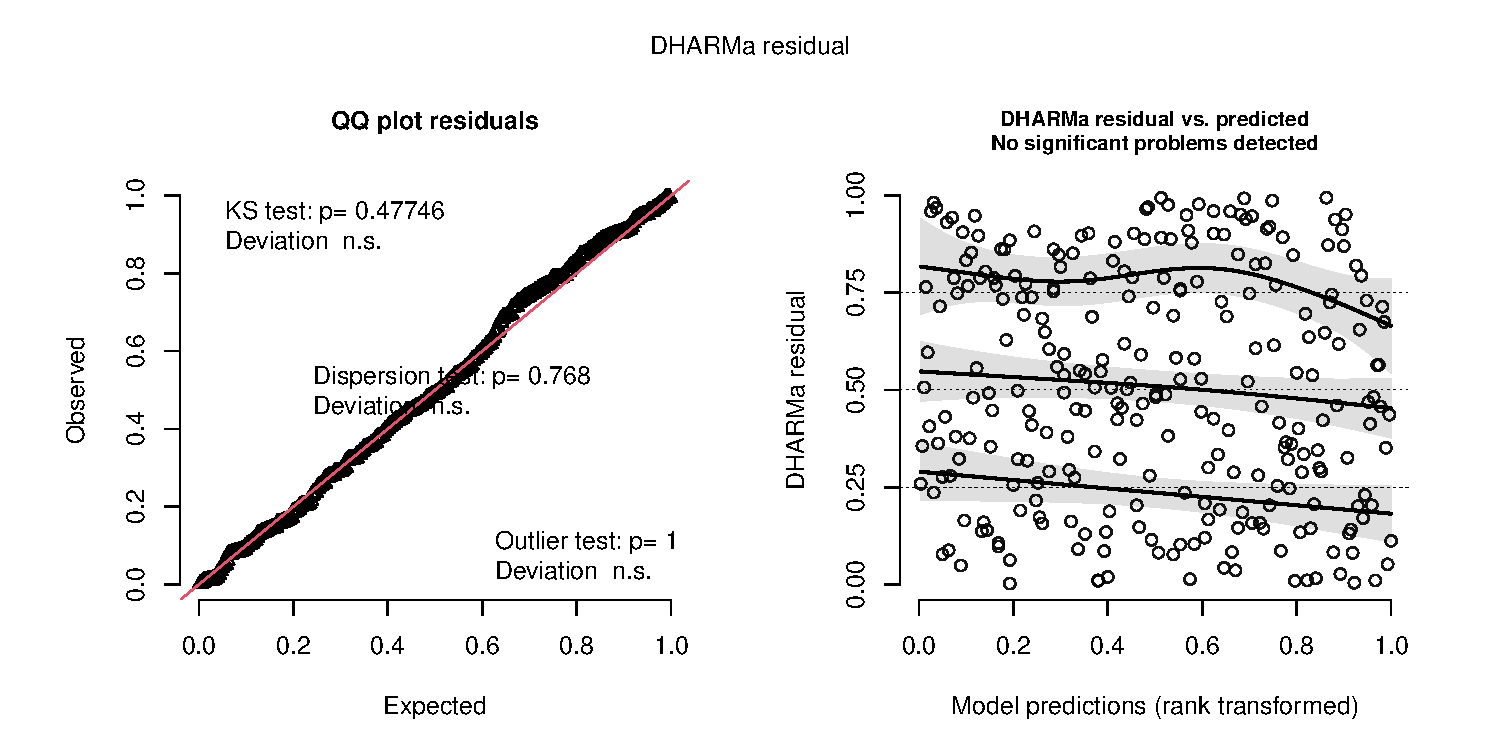
\includegraphics[keepaspectratio]{final_files/figure-pdf/unnamed-chunk-6-1.pdf}}

\subsection{\texorpdfstring{\textbf{h. Visualize the model
predictions}}{h. Visualize the model predictions}}\label{h.-visualize-the-model-predictions}

\begin{Shaded}
\begin{Highlighting}[]
\NormalTok{mod\_int\_preds }\OtherTok{\textless{}{-}} \FunctionTok{suppressMessages}\NormalTok{(}
  \FunctionTok{ggpredict}\NormalTok{(mod\_int,}
            \AttributeTok{terms =} \FunctionTok{c}\NormalTok{(}\StringTok{"height\_cm"}\NormalTok{,}
                      \StringTok{"ant\_species\_full"}\NormalTok{)))}

\CommentTok{\#Convert predictions to data frame}
\NormalTok{mod\_int\_preds }\OtherTok{\textless{}{-}} \FunctionTok{as.data.frame}\NormalTok{(mod\_int\_preds)}

\CommentTok{\#Rename group column to match raw data}
\NormalTok{mod\_int\_preds }\OtherTok{\textless{}{-}}\NormalTok{ mod\_int\_preds }\SpecialCharTok{|\textgreater{}}
  \FunctionTok{rename}\NormalTok{(}\AttributeTok{ant\_species\_full =}\NormalTok{ group)}

\CommentTok{\#Plot model predictions and raw data}
\FunctionTok{ggplot}\NormalTok{() }\SpecialCharTok{+}
  
  \CommentTok{\#Add underlying data}
  \FunctionTok{geom\_jitter}\NormalTok{(}\AttributeTok{data =}\NormalTok{ nests\_clean,}
              \FunctionTok{aes}\NormalTok{(}\AttributeTok{x =}\NormalTok{ height\_cm,}
                  \AttributeTok{y =}\NormalTok{ case\_control,}
                  \AttributeTok{color =}\NormalTok{ ant\_species\_full),}
              \AttributeTok{width =} \DecValTok{0}\NormalTok{,}
              \AttributeTok{height =} \FloatTok{0.05}\NormalTok{,}
              \AttributeTok{alpha =} \FloatTok{0.5}\NormalTok{) }\SpecialCharTok{+}
  
  \CommentTok{\#Add confidence intervals around predictions and underlying data}
  \FunctionTok{geom\_ribbon}\NormalTok{(}\AttributeTok{data =}\NormalTok{ mod\_int\_preds,}
              \FunctionTok{aes}\NormalTok{(}\AttributeTok{x =}\NormalTok{ x,}
                  \AttributeTok{ymin =}\NormalTok{ conf.low,}
                  \AttributeTok{ymax =}\NormalTok{ conf.high,}
                  \AttributeTok{fill =}\NormalTok{ ant\_species\_full),}
              \AttributeTok{alpha =} \FloatTok{0.25}\NormalTok{) }\SpecialCharTok{+}
  
  \CommentTok{\#Add model prediction lines}
  \FunctionTok{geom\_line}\NormalTok{(}\AttributeTok{data =}\NormalTok{ mod\_int\_preds,}
            \FunctionTok{aes}\NormalTok{(}\AttributeTok{x =}\NormalTok{ x,}
                \AttributeTok{y =}\NormalTok{ predicted,}
                \AttributeTok{color =}\NormalTok{ ant\_species\_full),}
            \AttributeTok{linewidth =} \DecValTok{1}\NormalTok{) }\SpecialCharTok{+}
  
  \CommentTok{\#Create separate panels for each ant species}
  \FunctionTok{facet\_wrap}\NormalTok{(}\SpecialCharTok{\textasciitilde{}}\NormalTok{ ant\_species\_full) }\SpecialCharTok{+}
  
  \CommentTok{\#Change colors}
  \FunctionTok{scale\_color\_manual}\NormalTok{(}\AttributeTok{values =} \FunctionTok{c}\NormalTok{(}\StringTok{"firebrick"}\NormalTok{,}
                                \StringTok{"steelblue"}\NormalTok{,}
                                \StringTok{"forestgreen"}\NormalTok{)) }\SpecialCharTok{+}
  \FunctionTok{scale\_fill\_manual}\NormalTok{(}\AttributeTok{values =} \FunctionTok{c}\NormalTok{(}\StringTok{"firebrick"}\NormalTok{,}
                               \StringTok{"steelblue"}\NormalTok{,}
                               \StringTok{"forestgreen"}\NormalTok{)) }\SpecialCharTok{+}
  
  \CommentTok{\#Label axes in full}
  \FunctionTok{labs}\NormalTok{(}\AttributeTok{x =} \StringTok{"Tree height (cm)"}\NormalTok{,}
       \AttributeTok{y =} \StringTok{"Probability of nest occurrence"}\NormalTok{) }\SpecialCharTok{+}
  
  \CommentTok{\#Remove legend}
  \FunctionTok{theme\_classic}\NormalTok{() }\SpecialCharTok{+}
  \FunctionTok{theme}\NormalTok{(}\AttributeTok{legend.position =} \StringTok{"none"}\NormalTok{)}
\end{Highlighting}
\end{Shaded}

\pandocbounded{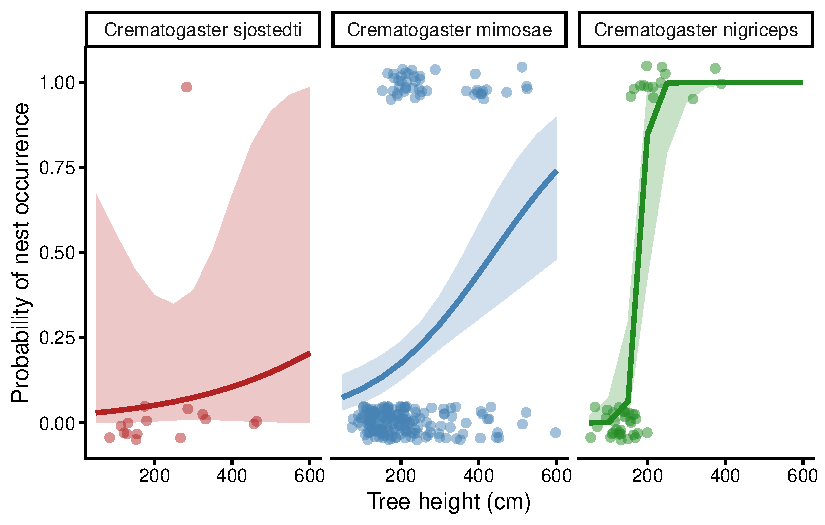
\includegraphics[keepaspectratio]{final_files/figure-pdf/unnamed-chunk-7-1.pdf}}

\subsection{\texorpdfstring{\textbf{i. Write a caption for your
figure}}{i. Write a caption for your figure}}\label{i.-write-a-caption-for-your-figure}

\textbf{Figure 1. Predicted probability of nest occurrence by tree
height and acacia ant species.} Points represent the underlying nest
occurrence data, where 1 indicates a tree containing a bird nest and 0
indicates an available and suitable tree that does not contain a bird
nest. The lines represent model predictions from the selected logistic
regression model, and surrounding lighter coloured shaded ribbons
represent the 95\% confidence intervals. Separate panels show
predictions for \emph{Crematogaster sjostedti} ( displayed in red),
\emph{Crematogaster mimosae} (displayed in blue), and
\emph{Crematogaster nigriceps} (displayed in green). Data are from
Lujan, E., Nielsen, R., Short, Z., Wicks, S., Nderitu Watetu, W.,
Malingati Khasoha, L., Palmer, T. M., Goheen, J. R., \& Alston, J. M.
(2023). Data, code, and metadata for: Symbiotic acacia ants drive
nesting behavior by birds in an African savanna
\url{https://doi.org/10.5281/zenodo.8373322}

\subsection{j. Calculate model
predictions}\label{j.-calculate-model-predictions}

\begin{Shaded}
\begin{Highlighting}[]
\CommentTok{\#Create new data for a tree height fixed at 600 cm}
\NormalTok{pred\_600 }\OtherTok{\textless{}{-}} \FunctionTok{tibble}\NormalTok{(}\AttributeTok{height\_cm =} \FunctionTok{c}\NormalTok{(}\DecValTok{600}\NormalTok{,}
                                 \DecValTok{600}\NormalTok{,}
                                 \DecValTok{600}\NormalTok{),}
                   \AttributeTok{ant\_species\_full =} \FunctionTok{factor}\NormalTok{(}\FunctionTok{c}\NormalTok{(}\StringTok{"Crematogaster sjostedti"}\NormalTok{,}
                                               \StringTok{"Crematogaster mimosae"}\NormalTok{,}
                                               \StringTok{"Crematogaster nigriceps"}\NormalTok{),}
                                             \AttributeTok{levels =} \FunctionTok{c}\NormalTok{(}\StringTok{"Crematogaster sjostedti"}\NormalTok{,}
                                                        \StringTok{"Crematogaster mimosae"}\NormalTok{,}
                                                        \StringTok{"Crematogaster nigriceps"}\NormalTok{)))}

\CommentTok{\#Calculate model predictions at 600 cm}
\NormalTok{pred\_600\_output }\OtherTok{\textless{}{-}} \FunctionTok{predict}\NormalTok{(mod\_int,}
                           \AttributeTok{newdata =}\NormalTok{ pred\_600,}
                           \AttributeTok{type =} \StringTok{"link"}\NormalTok{,}
                           \AttributeTok{se.fit =} \ConstantTok{TRUE}\NormalTok{)}

\CommentTok{\#Create table by converting predictions from log{-}odds into probabilities}
\NormalTok{pred\_600\_table }\OtherTok{\textless{}{-}}\NormalTok{ pred\_600 }\SpecialCharTok{|\textgreater{}}
  \FunctionTok{mutate}\NormalTok{(}\AttributeTok{predicted\_probability =} \FunctionTok{plogis}\NormalTok{(pred\_600\_output}\SpecialCharTok{$}\NormalTok{fit),}
         \AttributeTok{conf\_low =} \FunctionTok{plogis}\NormalTok{(pred\_600\_output}\SpecialCharTok{$}\NormalTok{fit }\SpecialCharTok{{-}} \FloatTok{1.96} \SpecialCharTok{*}\NormalTok{ pred\_600\_output}\SpecialCharTok{$}\NormalTok{se.fit),}
         \AttributeTok{conf\_high =} \FunctionTok{plogis}\NormalTok{(pred\_600\_output}\SpecialCharTok{$}\NormalTok{fit }\SpecialCharTok{+} \FloatTok{1.96} \SpecialCharTok{*}\NormalTok{ pred\_600\_output}\SpecialCharTok{$}\NormalTok{se.fit))}

\CommentTok{\#Display the predicted probabilities with all columns}
\NormalTok{pred\_600\_table }\SpecialCharTok{|\textgreater{}}
  
  \CommentTok{\#Show columns in order }
  \FunctionTok{select}\NormalTok{(ant\_species\_full,}
\NormalTok{         height\_cm,}
\NormalTok{         predicted\_probability,}
\NormalTok{         conf\_low,}
\NormalTok{         conf\_high)}
\end{Highlighting}
\end{Shaded}

\begin{verbatim}
# A tibble: 3 x 5
  ant_species_full        height_cm predicted_probability conf_low conf_high
  <fct>                       <dbl>                 <dbl>    <dbl>     <dbl>
1 Crematogaster sjostedti       600                 0.205 0.000970     0.986
2 Crematogaster mimosae         600                 0.741 0.481        0.898
3 Crematogaster nigriceps       600                 1     1.000        1    
\end{verbatim}

\subsection{k. Interpret your results}\label{k.-interpret-your-results}

When tree height is set to 600 cm, the model predicted that the
probability of nest occurrence was highest for trees inhabited by the
more aggressive \emph{Crematogaster nigriceps} at 1.000 (95\% CI: 1.000,
1.000), followed by the \emph{Crematogaster mimosae} at 0.741 (95\% CI:
0.481, 0.898), and was the lowest for the \emph{Crematogaster sjostedti}
at 0.205 (95\% CI: 0.001, 0.986). As displayed in Figure 1, the
relationship between tree height and probability of nest occurrence
differed depending on the type of acacia ant species present, with nest
occurrence increasing most strongly with height for trees inhabited by
the \emph{C. nigriceps} ants. Ultimately, nest occurrence was more
likely in that of taller trees and in trees inhabited by the more
aggressive ant defenders, such as \emph{C. nigriceps} and \emph{C.
mimosae}. Biologically speaking, this pattern may exist as aggressive
ant species better defend host trees from predators and disturbances,
making these trees better suited for nest selection.

\section{Problem 3. Affective and exploratory
visualizations}\label{problem-3.-affective-and-exploratory-visualizations}

\section{a. Comparing visualizations}\label{a.-comparing-visualizations}

The affective visualization was primarily inspired by the scatter plot
exploratory visualization examining the relationship between sleep
duration and productivity level. The heights of the buildings
represented sleep duration, while exposure to sunlight represented
productivity. The arrangement of the buildings follows the overall
trendline displayed in the scatter plot, allowing the affective
visualization to still effectively communicate the relationship between
the two variables but in a more visually compelling manner.

\section{b. Designing an analysis}\label{b.-designing-an-analysis}

A simple linear regression model may be used to answer my initially
proposed research question, ``How does the amount of sleep I get a night
affect my daily productivity?'' This analysis is appropriate as the
measured response variable, productivity level (measured as tasks
completed over tasks initially planned and expressed as a percentage),
and the predictor variable, sleep duration (measured in minutes), are
both continuous variables. This analysis would ultimately allow me to
determine if changes in my sleep duration are associated with changes in
my overall productivity level, and further articulate the strength and
direction of that relationship.

\subsection{c.~Check any assumptions and run your
analysis}\label{c.-check-any-assumptions-and-run-your-analysis}

\subsubsection{Check any assumptions}\label{check-any-assumptions}

\begin{Shaded}
\begin{Highlighting}[]
\CommentTok{\#Create productivity variable as percentage}
\NormalTok{my\_data\_clean }\OtherTok{\textless{}{-}}\NormalTok{ my\_data }\SpecialCharTok{|\textgreater{}}
  \FunctionTok{mutate}\NormalTok{(}\AttributeTok{productivity\_level =}\NormalTok{ tasks\_completed }\SpecialCharTok{/}\NormalTok{ tasks\_planned }\SpecialCharTok{*} \DecValTok{100}\NormalTok{)}

\CommentTok{\#Create linear model}
\NormalTok{sleep\_productivity\_mod }\OtherTok{\textless{}{-}} \FunctionTok{lm}\NormalTok{(productivity\_level }\SpecialCharTok{\textasciitilde{}}\NormalTok{ sleep\_minutes,}
                             \AttributeTok{data =}\NormalTok{ my\_data\_clean)}

\CommentTok{\#Check linearity and if variance is constant}
\FunctionTok{plot}\NormalTok{(sleep\_productivity\_mod, }\AttributeTok{which =} \DecValTok{1}\NormalTok{)}
\end{Highlighting}
\end{Shaded}

\pandocbounded{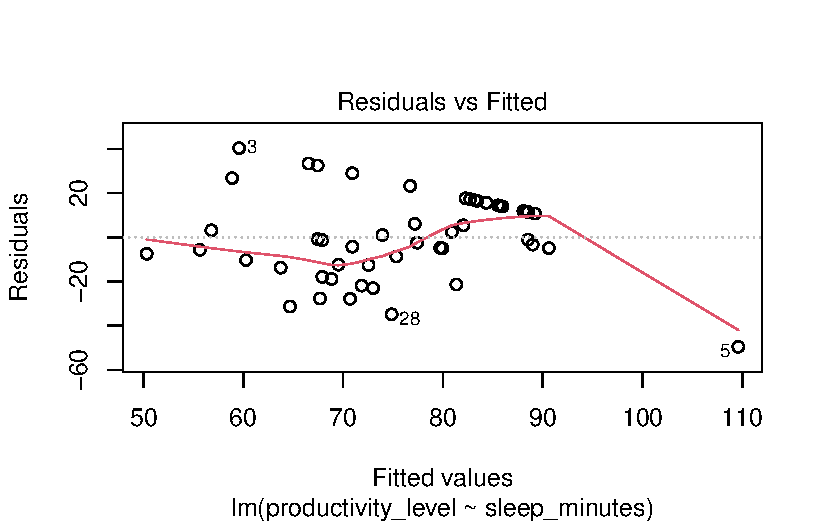
\includegraphics[keepaspectratio]{final_files/figure-pdf/unnamed-chunk-9-1.pdf}}

\begin{Shaded}
\begin{Highlighting}[]
\CommentTok{\#Check if residuals are normal}
\FunctionTok{plot}\NormalTok{(sleep\_productivity\_mod, }\AttributeTok{which =} \DecValTok{2}\NormalTok{)}
\end{Highlighting}
\end{Shaded}

\pandocbounded{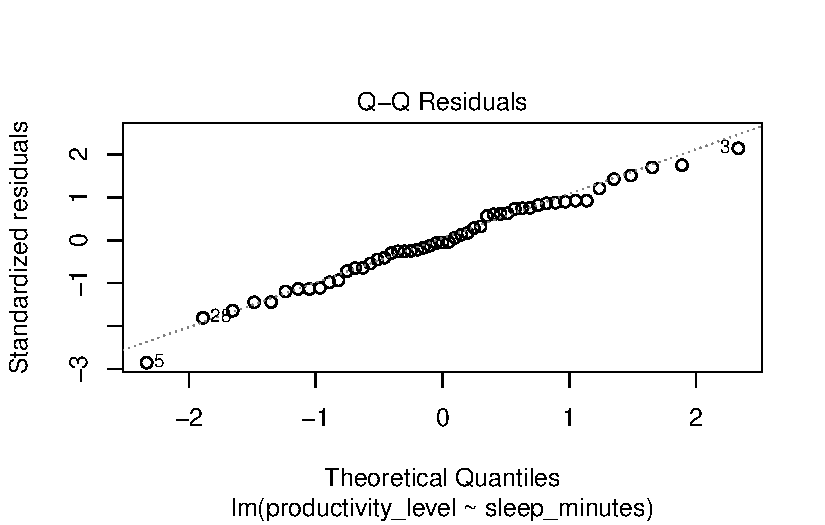
\includegraphics[keepaspectratio]{final_files/figure-pdf/unnamed-chunk-9-2.pdf}}

\subsubsection{Run the analysis proposed in part
b}\label{run-the-analysis-proposed-in-part-b}

\begin{Shaded}
\begin{Highlighting}[]
\CommentTok{\#Run simple the linear regression}
\FunctionTok{summary}\NormalTok{(sleep\_productivity\_mod)}
\end{Highlighting}
\end{Shaded}

\begin{verbatim}

Call:
lm(formula = productivity_level ~ sleep_minutes, data = my_data_clean)

Residuals:
    Min      1Q  Median      3Q     Max 
-49.608 -12.467  -1.028  14.368  40.428 

Coefficients:
               Estimate Std. Error t value Pr(>|t|)    
(Intercept)   -24.28496   24.85887  -0.977 0.333411    
sleep_minutes   0.23165    0.05724   4.047 0.000184 ***
---
Signif. codes:  0 '***' 0.001 '**' 0.01 '*' 0.05 '.' 0.1 ' ' 1

Residual standard error: 19.46 on 49 degrees of freedom
Multiple R-squared:  0.2505,    Adjusted R-squared:  0.2352 
F-statistic: 16.38 on 1 and 49 DF,  p-value: 0.0001836
\end{verbatim}

\subsubsection{Calculate an effect size}\label{calculate-an-effect-size}

\begin{Shaded}
\begin{Highlighting}[]
\CommentTok{\#Calculate effect size for linear regression}
\FunctionTok{summary}\NormalTok{(sleep\_productivity\_mod)}\SpecialCharTok{$}\NormalTok{r.squared}
\end{Highlighting}
\end{Shaded}

\begin{verbatim}
[1] 0.2505394
\end{verbatim}

\subsection{d.~Create a visualization}\label{d.-create-a-visualization}

\begin{Shaded}
\begin{Highlighting}[]
\CommentTok{\#Create a scatterplot to display relationship between sleep and productivity}
\FunctionTok{ggplot}\NormalTok{(}\AttributeTok{data =}\NormalTok{ my\_data\_clean,}
       \AttributeTok{mapping =} \FunctionTok{aes}\NormalTok{(}\AttributeTok{x =}\NormalTok{ sleep\_minutes,}
                     \AttributeTok{y =}\NormalTok{ productivity\_level)) }\SpecialCharTok{+}
  
  \CommentTok{\#Add one point for each daily observation from data set}
  \FunctionTok{geom\_point}\NormalTok{(}\AttributeTok{color =} \StringTok{"darkgreen"}\NormalTok{,}
             \AttributeTok{size =} \DecValTok{2}\NormalTok{,}
             \AttributeTok{alpha =} \FloatTok{0.75}\NormalTok{) }\SpecialCharTok{+}
  
  \CommentTok{\#Add linear regression trend line from analysis and 95\% confidence interval}
  \FunctionTok{geom\_smooth}\NormalTok{(}\AttributeTok{method =} \StringTok{"lm"}\NormalTok{,}
              \AttributeTok{se =} \ConstantTok{TRUE}\NormalTok{,}
              \AttributeTok{color =} \StringTok{"black"}\NormalTok{,}
              \AttributeTok{fill =} \StringTok{"lightgreen"}\NormalTok{) }\SpecialCharTok{+}
  
  \CommentTok{\#Relabel both axes}
  \FunctionTok{labs}\NormalTok{(}\AttributeTok{x =} \StringTok{"Sleep (minutes)"}\NormalTok{,}
       \AttributeTok{y =} \StringTok{"Productivity level (\%)"}\NormalTok{,}
       \AttributeTok{title =} \StringTok{"Productivity versus Sleep"}\NormalTok{) }\SpecialCharTok{+}
  
  \CommentTok{\#Set x{-}axis tick marks}
  \FunctionTok{scale\_x\_continuous}\NormalTok{(}\AttributeTok{breaks =} \FunctionTok{seq}\NormalTok{(}\DecValTok{300}\NormalTok{,}
                                \DecValTok{600}\NormalTok{,}
                                \AttributeTok{by =} \DecValTok{50}\NormalTok{)) }\SpecialCharTok{+}
  \CommentTok{\#Change theme}
  \FunctionTok{theme\_light}\NormalTok{() }\SpecialCharTok{+}
  
  \CommentTok{\#Center title}
  \FunctionTok{theme}\NormalTok{(}\AttributeTok{plot.title =} \FunctionTok{element\_text}\NormalTok{(}\AttributeTok{hjust =} \FloatTok{0.5}\NormalTok{))}
\end{Highlighting}
\end{Shaded}

\begin{verbatim}
`geom_smooth()` using formula = 'y ~ x'
\end{verbatim}

\pandocbounded{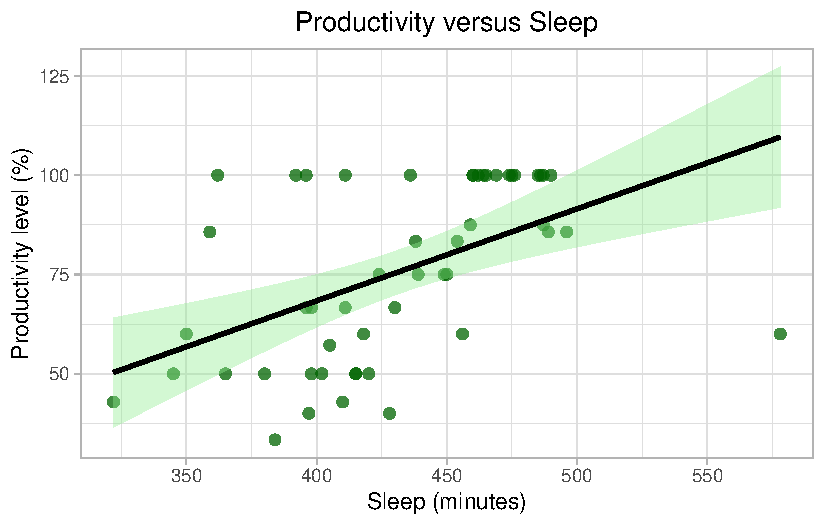
\includegraphics[keepaspectratio]{final_files/figure-pdf/unnamed-chunk-12-1.pdf}}

\subsection{e. Write a caption}\label{e.-write-a-caption}

\textbf{Figure 2. Relationship between sleep duration and productivity
level.} Green points represent daily observations, derived from my
personal data set, where sleep duration is measured in minutes slept
each night and productivity level is measured as tasks completed divided
by tasks planned, expressed as a percentage. The black line displays the
predicted relationship from the simple linear regression model, and the
surrounding light green shaded ribbon represents the 95\% confidence
interval. Data are from my personal data collected in ENVS 193DS at UCSB
during Spring 2026.

\subsection{f.~Write about your
results}\label{f.-write-about-your-results}

A simple linear regression model was used to analyze the relationship
between sleep duration and productivity level. The relationship was
found to be statistically significant (simple linear regression, F(1,
49)=16.38, p\textless0.001, \(\alpha = 0.05\), R²=0.251), with sleep
duration explaining around 25.1\% of the variation seen in productivity
level. As displayed in Figure 2, an increase in productivity level
coincided with an increase in sleep duration, with each additional
minute of sleep predicting an increase of 0.232 percentage points in
productivity level.




\end{document}
